\chapter{Introdução}
\label{chap:intro}

A tecnologia tem perpetrado cada vez mais diversas áreas do saber, trazendo diversos benefícios e praticidades a vida contemporânea. Destas diferentes áreas, uma das que mais se beneficiaram com a tecnologia e a inovação foi a área médica. Desde meados dos anos 2000, a quantidade de dados disponível vêm crescendo exponencialmente se alcançando uma projeção de centenas de milhares de \gls{EB} para os anos de 2020 em diante \cite{gantzDIGITALUNIVERSE2020}.

A Medicina tem cada vez mais gerado dados, sejam textuais, clínicos ou de imagem, e se utilizado deles para comporem seus diagnósticos. Tanto a \gls{TC} quanto a \gls{RMC} são exemplos de exames que podem gerar objetos tridimensionais (3D) de estruturas específicas do corpo humano a partir de dezenas de fatias que representam de forma bidimensional (2D), determinada estrutura do corpo humano dado um instante de tempo $t$. A \gls{IA} emergiu como uma das principais inovações no campo da imagem diagnóstica, com um impacto substancial em toda área médico inclusiva coma análises de \gls{RMC}. A \gls{IA} estará cada vez mais presente no mundo médico, com forte potencial para maior eficiência e precisão diagnóstica \cite{argentieroApplicationsArtificialIntelligence2022}.


A IA, tem como um de seus componentes as redes neurais profundas, também conhecido como \gls{AP}. O \gls{AP} é utilizado para resolver problemas do espectro de visão computacional, como: classificadores de imagens, detectores de objetos, segmentadores, etc. Estas redes, com suas múltiplas camadas profundas, geram características discriminantes após otimizadas a cerca de um conjunto de dados. Outro modelo de rede que vem tendo um uso cada vez maior e se encontra em diversas arquiteturas atuais, são as redes \textit{transformers}. As redes \textit{transformers} ficaram populares por serem comumente usadas em redes generativas auto-regressivas para geração sintética de texto, também conhecidas como \gls{LLM}, tendo como como seu exemplo mais conhecido o \textit{ChatGPT}. Os \textit{transformers} são arquiteturas que possuem como ponto forte principalmente sua capacidade de paralelismo e seu mecanismo de auto-atenção que permite que o modelo se concentre nas partes relevantes dos dados de entrada, aprimorando a compreensão do contexto e das relações dentro os dados \cite{russell2020artificial}.

Outras técnicas de processamento de imagem como análise de textura vem sendo utilizadas por várias décadas em diversos domínios da medicina. Em oncologia, a análise de textura de imagens de \gls{TC} mostrou correlação com a biologia tumoral subjacente, ao analisar características histológicas diferentes e mutações genéticas específicas. A biologia tumoral subjacente representam mecanismos biológicos fundamentais que estão na base do desenvolvimento, crescimento e progressão de tumores. Em problemas de tumores malignos já bem estabelecidos, a análise de textura se relaciona com a histologia do tumor em muitos tumores sólidos comuns (pulmão, colorretal, esofágico, mama), ela se correlaciona com mutações genéticas específicas e pode acompanhar respostas terapêuticas. Fora da oncologia, mudanças não malignas em órgãos podem ser detectadas, sendo exemplos cirrose hepática e pneumonite intersticial usual. Dentro do domínio de análise de imagens cardíacas, a análise de textura aplicada à \gls{RMC} tem sido usada para avaliar o risco de arritmia pós-infarto do miocárdio, o uso da RMC em imagens sem contraste e com realce tardio de gadolínio em pacientes com \gls{CMH} para prever o resultado é uma área de interesse particular atualmente \cite{schofieldTextureAnalysisCardiovascular2019a}.

% -----------------------------------------
% @TODO  - pg 11
% 1) o uso da RMC ou o uso de analise de textura em RMC para detectar cardiomiopatia hipertrofica?

% 2) e a cardiomiopatia dilatada?

% 3) Ao longo de cada frase precisa de uma citação, esse schoffield é para todas? Sugiro variar pelo menos com mais uma. 

% 4) o artigo é de 2019 e vc fala que é uma area de interesse atual.. mas isso é 5 anos atras. rever.
%-----------------------------------------

Uma área que se utiliza desse tipo de técnica é a análise radiômica que consiste no processo em obter dados qualitativos destas imagens de radiografias combinadas, e por vezes, a extração também da textura destas \cite{lambinRadiomicsExtractingMore2012}. A análise radiômica pode até ser usada para avaliar a resposta ao tratamento ou para transmitir certas características prognósticas. Dentre as doenças do coração, a \gls{CMH} é desenvolvida prioritariamente em jovens e pessoas de meia idade, sendo a mais comum das cardiomiopatias . Mesmo que a \gls{CMH} se apresente de forma assintomática em parte dos casos, esta pode culminar em morte súbita cardíaca, insuficiência cardíaca, acidente vascular cerebral e arritmia . A análise radiômica auxilia com o diagnóstico prévio afim de compreender e atuar nos casos de \gls{CMH} que demonstrem risco ao paciente \cite{kwonComparisonMortalityCause2022}.

%-----------------------------------------
% @TODO - pg 11
% Aqui eu comentaria algo assim: que pode atuar no diagnóstico de diversas doenças, como a cardiomiopatia que consiste... (definir em 1 linha e colocar citação) e possui diversos tipos, destacando-se a CMD e CMH, que ocorrem com mais frequência na população mundial (citar).
%-----------------------------------------

% Algumas de suas características são: extração de características, quantificação e padronização, possibilidade de correlação com dados clínicos. As aplicações da análise radiômica consiste em diversas aplicações clínicas, incluindo diagnóstico auxiliado por computador, predição de resposta ao tratamento, estratificação de pacientes, identificação de biomarcadores e personalização de tratamentos.

A análise radiômica em conjunto com técnicas de \gls{IA} tem um grande potencial e há pesquisas que já tentam unificar estes dois campos. O trabalho de \citeonline{aiSelfAttentionBasedFusion2023}, propôs a unificação de características radiômicas e características profundas, assim chamadas por serem extraídas de um modelo de \gls{AP}. Um modelo utilizando do mecanismo de auto-atenção para analisar e prever \gls{CMH}, uma vez as características unificadas também foi proposto. O uso destas duas abordagens aliadas na extração de características a cerca da doença, tem o potencial de obter melhores resultados preditivos se comparados as técnicas isoladas. A arquitetura proposta é conferida na Figura \ref{fig:fig006}. Os resultado deste trabalho obtiveram acurácia de $82,35\%$ e AUC de $0,74$.

\begin{figure}[ht]
    \centering
    \captionsetup{justification=centering}
    \caption{Arquitetura Proposta}
    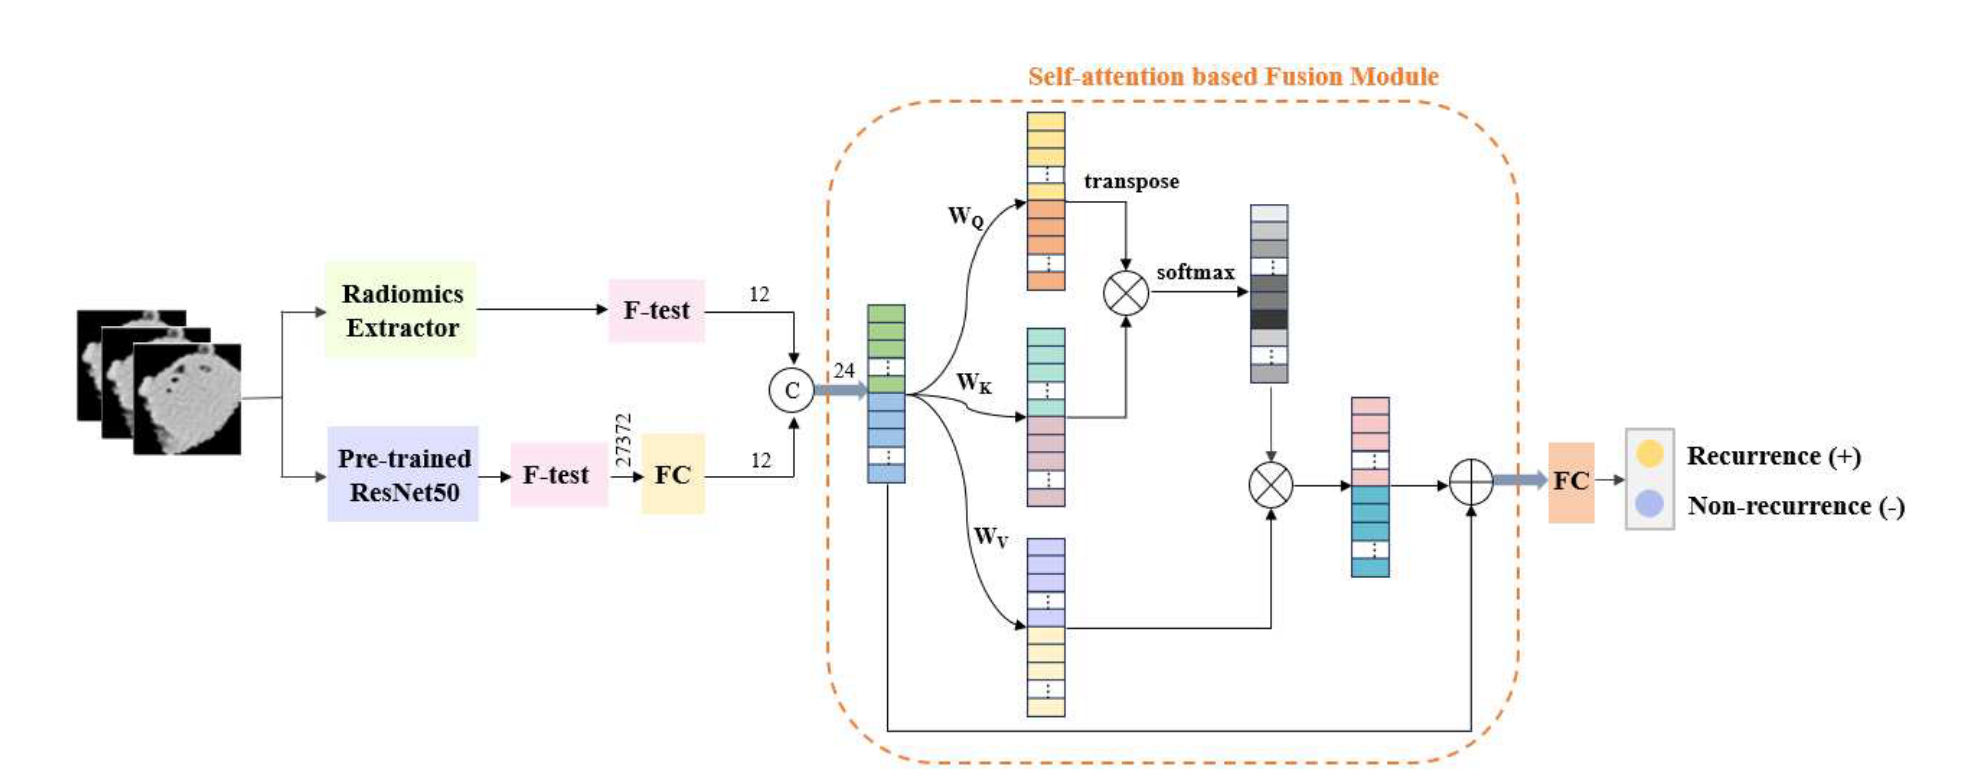
\includegraphics[width=1\textwidth]{figures/fig006.png}
    \caption*{Fonte: \cite{aiSelfAttentionBasedFusion2023}}
    \label{fig:fig006}
\end{figure}



% \newpage
\clearpage

%---------------------------------------------------------
\section{Objetivo}
\label{sec:cap1_objetivo}

No presente trabalho, será proposto 

Dado o contexto na qual o presente projeto de pesquisa está inserido, o objetivo geral deste trabalho é implementar e validar uma estratégia de fusão que combina as características manuais extraídas da análise de textura radiômica e características profundas, para melhorar a expressividade e a habilidade de generalização do modelo de \gls{RNP}. Será utilizado imagens de \gls{RMC} e as doenças \gls{CMH} e \gls{CMD} como objetos de estudo para avaliar o desempenho da abordagem. Como objetivos específicos, têm-se:

\begin{enumerate}

\item Modelo, que utiliza características radiômicas e
características profundas.

\item Coleta de resultados em conjunto de dados públicos, como linha de base da análise.

\item Avaliação dos resultados iniciais.

\item Proposta de novas abordagens tanto no pré-processamento quanto na arquitetura, mediante coleta dos resultados.

\item Iteração e análise dos resultados obtidos, sua documentação e comparação.
\end{enumerate}

%---------------------------------------------------------
\section{Estrutura do trabalho}
\label{sec:cap1_estrutura_trabalho}

Esta proposta está organizada em seis capítulos, a saber:
O \textbf{Capítulo \ref{chap:intro}} apresenta a introdução, objetivo e contribuições desejadas. O \textbf{Capítulo \ref{chap:fundamentacao_teorica}} faz um aprofundamento teórico no tema de pesquisa estudando as técnicas consideradas primordiais deste trabalho e/ou que são utilizadas no desenvolvimento do experimento prático. No \textbf{Capítulo \ref{chap:trab_relacionados}} é estudado  os trabalhos recentes, não superior a cinco anos passados, de outros autores que estão de alguma forma relacionados com tema, sendo estes trabalhos relacionados oriundos de uma minuciosa revisão sistemática da literatura. No \textbf{Capítulo \ref{chap:metodologia}} é apresentada uma proposta de metodologia para a realização do experimento prático. O \textbf{Capítulo \ref{chap:proposta_experimental}} é uma proposta experimental que contempla os dados utilizados, informações do seu pré-processamento, hiperparâmetros planejados e demais informações assim como o cronograma do presente projeto de pesquisa. No \textbf{Capítulo \ref{chap:resultados_discussao}}, são apresentados os resultados parciais da prova de conceitos, considerando a arquitetura proposta no artigo que serviu como base. Finalmente, o \textbf{Capítulo \ref{chap:conclusao}} apresenta conclusão do presente projeto de pesquisa.
